\documentclass{article}
\usepackage[utf8]{inputenc}
\usepackage[russian]{babel}
\usepackage{graphics}
\usepackage{amsfonts}
\usepackage{amssymb}

\ifx\pdfoutput\undefined
\usepackage{graphicx}
\else
\usepackage[pdftex]{graphicx}
\fi

\hoffset -2.0cm	
\voffset -3.0cm
\textheight 23.5cm 
\textwidth 17.0cm

\title{\bf Лемма о связности графа плохих симплексов}
\author{Амосов Федор}

\begin{document}
	\maketitle

    \paragraph{Лемма\\}
        \begin{itemize}
            \item Пусть дан набор $d$--мерных точек $P$, в котором любые $d + 2$ точки не лежат на одной $d$--мерной сфере, и дана точка $q$ вне $Conv P$.
            \item Рассмотрим $D$ --- симплексикацию Делоне набора точек $P$.  Построим на симплексах из $D$ следующий граф $G$. Его вершинами будут симплексы и еще одна выделенная вершина $t$. Между двумя различными симплексами будет ребро, если у них общая сторона, между симплексом и $t$ будет ребро, если симплекс является граничным (хотя бы одна его сторона является стороной $Conv P$).
            \item Назовем симплекс из $D$ {\it плохим}, если его описанный шар содержит внутри точку $q$. Рассмотрим подграф $G'$ --- граф $G$, индуцированный на плохие симплексы и на вершину $t$.
            \item Утверждение: граф $G'$ связен.
        \end{itemize}
        
        \begin{center}
            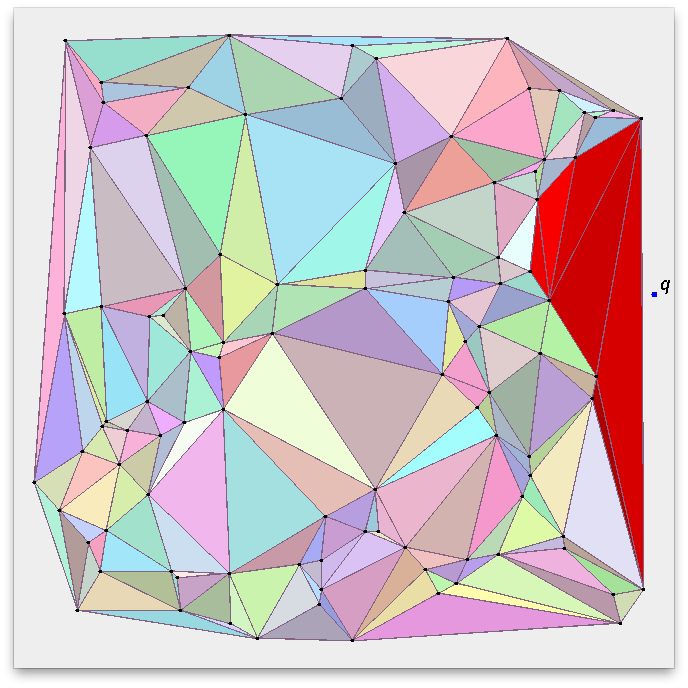
\includegraphics[scale=0.45]{1.png} 
                   
        \end{center}
        
        Черные точки --- точки $P$. Треугольники --- симплексы из $D$. Плохие треугольники (вершины графа $G'$) покрашены в красный цвет. Утверждается, что от любого красного треугольника можно дойти до границы по красным треугольникам.
        
    \paragraph{Доказательство\\}
        Пусть симплекс $S_0$ является плохим. Если мы докажем, что от $S_0$ можно дойти до границы по плохим симплексам, то мы докажем Лемму. Если $S_0$ граничный, то все ясно. Пусть $S_0$ не граничный симплекс. 
        
        Итак рассмотрим симплекс $S_0$. Обозначим за $d_0$ расстояние от $q$ до $S_0$ ($q \notin S_0$), а за $B_0$ --- описанный шар симплекса $S_0$. Симплекс $S_0$ плохой, значит $B_0$ содержит внутри точку $q$. Т.к. точка $q$ лежит вне $Conv P$, то $q \notin S_0$. Симплекс $S_0$ делит $B_0$ своими гранями на $d + 1$ сегмент. В одном из сегментов лежит точка $q$. Соответствующая грань $F$ является стороной некоторого симплекса $S_1 \neq S_0$, т.к. $S_0$ не граничный. $S_0$ и $S_1$ являются соседями в графе $G$. 
        
        Покажем, что $S_1$ так же плохой симплекс, т.е. докажем что описанный шар $B_1$ симплекса $S_1$ содержит внутри $q$. Обозначим за $p$ вершину $S_1$, не лежащую на грани $F$. Т.к. $S_0$ --- часть симплексикации Делоне, то точка $p$ лежит вне $B_0$.
        
        Итого, что у нас есть,
        \begin{itemize}
            \item $q$ внутри $B_0$
            \item $p$ снаружи $B_0$
            \item $p$ на границе $B_1$
            \item вершины $F$ лежат на $B_0$ и $B_1$
            \item $q$ и $p$ в одной полуплоскости относительно $F$ 
            \item $q$ внутри $B_1$ --- ?
        \end{itemize}

        \begin{center}
            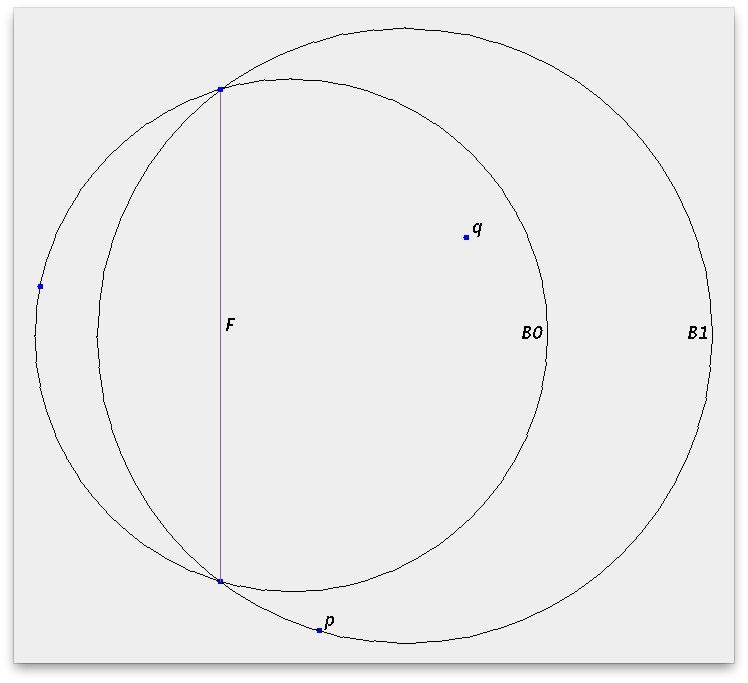
\includegraphics[scale=0.45]{2.png}       
        \end{center}
        
        Будем <<надувать>> (сдувать) шарик $B_0$ из <<кольца>> $F$, чтобы получился шарик $B_1$. Обозначим промежуточную стадию шара за $B$ (в начале, $B = B_0$, в конце, $B = B_1$). При надувании, в одной полуплоскости относительно $F$ точки будут только выходить из $B$, а в другой --- только входить в $B$. Тем самым, при надувании $B_0$ до $B_1$ точка $q$ будет оставаться в $B$. Мы будем надувать $B$ до тех пор, пока на его границе не окажется точка $p$. Тогда $B$ будет равно $B_1$. Тем самым, $q$ будет внутри и $B_1$.
        
        \begin{center}
            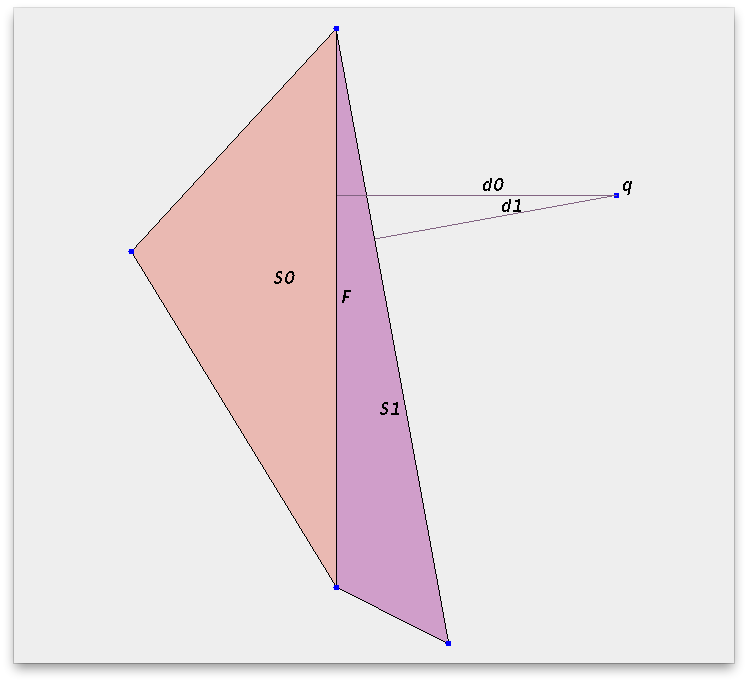
\includegraphics[scale=0.45]{3.png}       
        \end{center}        
        
        Расстояние от точки $q$ до симплекса $S_i$ есть расстояние от $q$ до грани $S_i$, соответствующей сегменту $B_i$, содержащему $q$. Очевидно, что расстоянию от $q$ до $S_1$ будет соответствовать грань, не равная $F$, но грань $F$ присутствует в $S_1$, поэтому расстояние от $q$ до $S_1$  $:= d_1 < dist(q, F) = d_0$. Тем самым, $d_0 > d_1$.
        
        Итак, мы из $S_0$ перешли по ребру графа $G'$ в плохой симплекс с меньшим расстоянием до $q$. Будем повторять такой переход, пока можем. Получим последовательность соседних плохих симплексов $S_0, S_1, S_2 \dots$ с расстояниями до $q$, $d_0 > d_1 > d_2 > \dots$ В такой цепочке симплексы не повторяются ввиду того, что их расстояния до $q$ не повторяются. Но симплексов конечное число, значит такая цепочка не может быть бесконечной. Рассмотрим последний симплекс $S_n$. Мы не можем из него перейти, значит он граничный (поскольку это было единственное предположение для перехода), ч.т.д.
        
      
    
        
              
         
	
\end{document}